\documentclass[11pt]{article}
\usepackage{amsmath,amssymb,graphicx,hyperref}
\usepackage[margin=2.6cm]{geometry}

\title{A no-go for perturbative baryogenesis in cosmologies with a bounded
thermal history}
\author{O.~Kirichenko}
\date{Draft skeleton --- \today}

\begin{document}
\maketitle

\begin{abstract}
We show that in any cosmology whose entire thermal history satisfies
$T \le T_{\max} \lesssim 130$~GeV --- bounce models with a QCD-scale
density cap, low-reheating scenarios, and cyclic models --- the baryon
asymmetry cannot be generated by perturbative baryon-number-violating
interactions of the thermal bath. For the representative dimension-six
operator $(qqq\ell)/\Lambda^2$, cosmological relevance at
$T_{\max} \sim \Lambda_{\rm QCD}$ requires $\Lambda \lesssim 3\times10^{6}$~GeV
even with a maximal thermal chemical-potential bias
($\epsilon_{\min} = 1.4\times10^{-9}$), while proton stability
($\tau_{p\to e^+\pi^0} > 2.4\times10^{34}$~yr) requires
$\Lambda \gtrsim 3\times10^{16}$~GeV: a gap of ten orders of magnitude in
$\Lambda$, i.e.\ forty orders in $\tau_p$. We further show that
environmental ``gating'' of the operator cannot rescue it: power-law
gates tied to the chiral condensate cannot bridge the required
$10^{-22}$ amplitude suppression and are turned \emph{on} inside
nucleons in bag-like descriptions, while derivative (phase-velocity)
gates are radiatively unstable. The surviving mechanisms are classified
exhaustively: (i) $B\!-\!L$-conserving transfer to a dark sector with
kinematic nucleon protection (asymmetric-dark-matter/mesogenesis class),
(ii) condensate-carried baryon number (Affleck--Dine class), and
(iii) non-thermal populations with $E \gg T_{\max}$ (heavy-relic decay,
collision-induced sphalerons, black-hole evaporation). As a corollary,
published bounce-baryogenesis scenarios that assume equilibrium
$B$-violation below the sphaleron threshold are excluded unless recast
in one of these three classes; in cyclic bounded-$T$ models a primordial
asymmetry is additionally excluded by entropy dilution, forcing
per-cycle regeneration.
\end{abstract}

\section{Introduction}
% - Sakharov conditions; the third condition is usually supplied by
%   sphalerons (T > 130 GeV) or GUT-scale physics.
% - A class of cosmologies never reaches those temperatures:
%   * low reheating scenarios [Davidson-Kolb PRL 84 (2000) 4284,
%     hep-ph/0001301; moduli reheating arXiv:1005.2804];
%   * bounce models with density caps at the QCD scale;
%   * cyclic models (temperature capped every cycle).
% - Existing bounce-baryogenesis literature [arXiv:2010.04807,
%   arXiv:2001.04773] assumes B-violating operators in equilibrium at
%   the bounce with a free decoupling temperature. This paper shows that
%   assumption is excluded by proton stability, quantitatively.
% - Structure of the paper.

\section{Setup and the theorem}
\subsection{Bounded thermal histories}
% Definition: T(t) <= T_max for all t, with T_max < T_sph ~ 130 GeV.
% Sphalerons: rate ~ exp(-E_sph/T), E_sph ~ 9 TeV -> exponent -21,000 at
% T = 432 MeV. Leptogenesis/GUT: unavailable in principle.

\subsection{The EFT window}
The lowest-dimension $\Delta B \neq 0$ operator,
$\mathcal{O}_6 = (qqq\ell)/\Lambda^2$, has thermal rate
$\Gamma \sim T^5/\Lambda^4$. Cosmological relevance requires
$\Gamma/H \ge \epsilon$ with the efficiency floor set by the maximal
thermal bias $\mu \sim \pi T$ (spontaneous baryogenesis
\`a la Cohen--Kaplan):
\begin{equation}
  \epsilon_{\min} = \frac{\eta_{\rm obs}}{\eta_{\rm eq}^{\max}}
  = \frac{8.6\times10^{-11}}{45/(12\pi g_*)} = 1.4\times10^{-9},
  \qquad
  \Lambda \le \Lambda_{\rm viab}(T_{\max})
  = \left(\frac{T_{\max}^3 M_{\rm Pl}}{1.66\sqrt{g_*}}\right)^{1/4}
    \epsilon_{\min}^{-1/4}.
\end{equation}
Proton stability requires
$\Lambda \ge \Lambda_p = (\tau_{\rm SK}\, m_p^5)^{1/4} = 3.0\times10^{16}$~GeV.
At $T_{\max} = 432$~MeV, $\Lambda_{\rm viab} = 3.1\times10^{6}$~GeV: the
windows are separated by $10^{10}$ in $\Lambda$ (Fig.~\ref{fig:excl}).
The ``EFT desert'' closes only at $T \sim 10^{13}$~GeV --- academically,
since the SM's own sphalerons rescue baryogenesis already above
$\sim 130$~GeV. % (this recovers the standard lore: viable baryogenesis
% lives either at sphalerons or at GUT scales; the intermediate EFT
% desert is proton-forbidden.)

\begin{figure}[t]
\centering
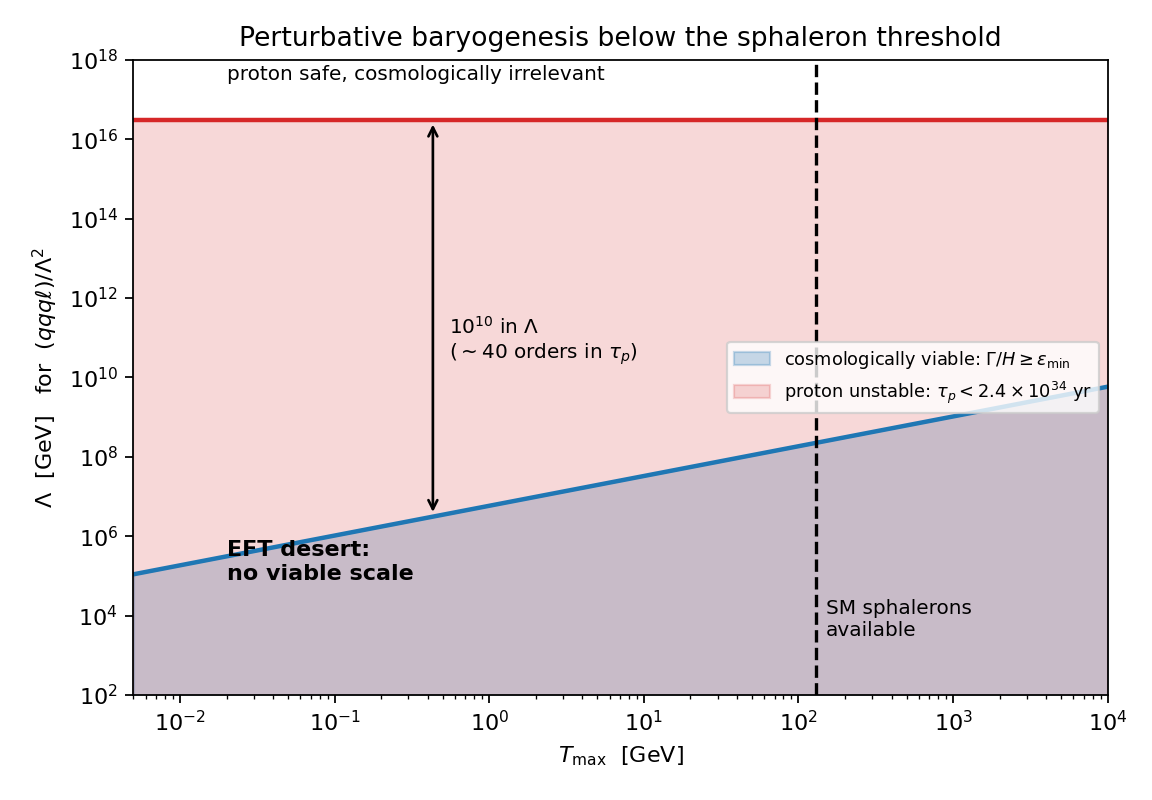
\includegraphics[width=0.82\textwidth]{fig_exclusion.png}
\caption{The $(T_{\max}, \Lambda)$ plane for $(qqq\ell)/\Lambda^2$.
Blue: cosmologically capable of generating $\eta_B$ under a maximal
thermal bias. Red: proton lifetime below the Super-Kamiokande bound.
The regions never meet below the sphaleron threshold (dashed).}
\label{fig:excl}
\end{figure}

\section{Gating does not help}
\subsection{Environmental (condensate) gates}
% (1 - W^2/W_0^2)^n type coefficients: in-medium condensate suppression
% inside nucleons is only ~25-30%, so bridging the required 1e-22
% amplitude needs n ~ 40 powers — outside EFT; and in bag-like hadron
% interiors the condensate is restored (gate fully ON inside the proton:
% the wrong direction). Numbers from the companion computation.

\subsection{Derivative gates are radiatively unstable}
% (\partial\theta)^2/M^2 * O_6: vacuum fluctuations
% <(\partial\theta)^2> ~ f^2/(16 pi^2) exceed any natural normalization
% M^2 = m_theta^2, regenerating the ungated operator with an O(100)
% coefficient. No symmetry distinguishes the gated from the ungated
% operator (both shift-symmetric), so the cancellation is a fine-tuning.
% cf. one-loop PQ proton decay arXiv:2607.02026 for a related mechanism.

\section{The surviving mechanisms}
\subsection{Class I: $B\!-\!L$-conserving dark transfer}
% Neutron-portal cogenesis: (udd)\chi/\Lambda^2 with total B-L = 0;
% proton safety BY SYMMETRY + kinematic corridor
%   m_n - S_n(Be-9) < m_chi < m_p + m_e  (937.90 - 938.78 MeV);
% benchmark: Lambda ~ 1e3 TeV, Br(n -> chi gamma) ~ 1e-7..1e-6 floor.
% Established relatives: ADM [Kaplan-Luty-Zurek], B-mesogenesis
% [Elor-Escudero-Nelson arXiv:1810.00880; collider roadmap 2101.02706].
% Note mesogenesis also invokes Class III (a heavy relic Phi).

\subsection{Class II: condensate-carried baryon number (Affleck--Dine)}
% Evades the theorem because the asymmetry is generated by coherent
% field dynamics, not thermal operators; requires a B-charged scalar
% with large initial displacement. In bounded-T cosmologies the
% displacement mechanism must be specified (no high-T epoch to set it).

\subsection{Class III: non-thermal high-energy populations}
% - heavy-relic decay (moduli at T_RH ~ 200 MeV [arXiv:1005.2804]);
% - collision sphalerons E_cm > E_sph [PRD 107, 015001];
% - PBH evaporation.
% Common requirement: a population with E >> T_max must be justified
% within the bounded-T history — nontrivial in cyclic models (below).

\section{Corollary: cyclic bounded-$T$ cosmologies}
% Inheritance of eta_B is excluded by entropy dilution: comoving B
% conserved, comoving S grows by factor g per cycle => eta ~ g^{-n};
% for g = 2, n = 77: suppression 2^76 ~ 1e23 -> requires eta_1 > 1e12,
% unphysical. Heavy relics likewise dilute; Class III requires per-cycle
% regeneration of the non-thermal population itself. Hence cyclic
% QCD-bounce models must realize Class I or II *every cycle*.

\section{Discussion}
% - Which published scenarios are affected: gravitational/spontaneous
%   baryogenesis in bounces [2010.04807, 2001.04773] — their assumed
%   B-violating decoupling temperature below the sphaleron threshold
%   places them in the excluded EFT desert unless recast as Class I-III.
% - Falsifiability of Class I: the neutron dark-decay floor.
% - Limitations: Gaussian rate estimates; O(1) factors; the bias ceiling.

\section*{Acknowledgments}
% Verification code: github.com/infosave2007/vmf (verification/ scripts
% nvg_baryogenesis_bsm_closure.py, nvg_adm_bl_cogenesis.py,
% nvg_etab_inheritance.py; figure: papers/bounded_T_nogo/).

\begin{thebibliography}{99}
\bibitem{DavidsonKolb} S.~Davidson, M.~Losada, A.~Riotto,
``Baryogenesis at low reheating temperatures,''
Phys.\ Rev.\ Lett.\ 84 (2000) 4284, hep-ph/0001301.
\bibitem{Moduli} R.~Allahverdi et al., ``Baryogenesis and late-decaying
moduli,'' arXiv:1005.2804.
\bibitem{QuantumBounce} ``Baryogenesis in cosmological models with
symmetric and asymmetric quantum bounces,'' arXiv:2010.04807.
\bibitem{BigBounce} ``Big Bounce Baryogenesis,'' arXiv:2001.04773.
\bibitem{SuperK} Super-Kamiokande Collaboration, search for
$p \to e^+\pi^0$: $\tau > 2.4\times10^{34}$ yr.
\bibitem{CohenKaplan} A.~G.~Cohen, D.~B.~Kaplan, ``Thermodynamic
generation of the baryon asymmetry,'' Phys.\ Lett.\ B 199 (1987) 251.
\bibitem{KLZ} D.~E.~Kaplan, M.~A.~Luty, K.~M.~Zurek, ``Asymmetric dark
matter,'' Phys.\ Rev.\ D 79 (2009) 115016.
\bibitem{Mesogenesis} G.~Elor, M.~Escudero, A.~E.~Nelson,
``Baryogenesis and dark matter from $B$ mesons,'' Phys.\ Rev.\ D 99
(2019) 035031, arXiv:1810.00880.
\bibitem{MesogenesisCollider} G.~Alonso-\'Alvarez, G.~Elor, M.~Escudero,
``Collider signals of baryogenesis and dark matter from $B$ mesons,''
Phys.\ Rev.\ D 104 (2021) 035028, arXiv:2101.02706.
\bibitem{HighESphaleron} ``High energy sphalerons for baryogenesis at
low temperatures,'' Phys.\ Rev.\ D 107 (2023) 015001.
\bibitem{FornalGrinstein} B.~Fornal, B.~Grinstein, ``Dark matter
interpretation of the neutron decay anomaly,'' Phys.\ Rev.\ Lett.\ 120
(2018) 191801.
\end{thebibliography}

\end{document}
